\documentclass[a4paper,11pt,french]{report}
\usepackage[utf8]{inputenc}

\usepackage[T1]{fontenc}
\usepackage[francais]{babel}
\usepackage[top=1.5cm, bottom=2cm, left=1.5cm, right=1.5cm, includeheadfoot]{geometry} %pour les marges
\usepackage{float}
\usepackage{lmodern}
\usepackage{pgfplots}
\usepackage{tikz}   
\usepackage{tikz-uml}   
\usepackage{fancyhdr} % Required for custom headers
\usepackage{lastpage} % Required to determine the last page for the footer
\usepackage{extramarks} % Required for headers and footers
\usepackage{graphicx} % Required to insert images
\usepackage{tabularx, longtable}
\usepackage{color, colortbl}
\usepackage{amsmath}
\usepackage{mathtools}
\usepackage{amssymb}
\usepackage[toc,page]{appendix} 
\usepackage{eurosym}
\usepackage{rotating}
\usepackage{array}
%\usepackage{cmbright}
\usepackage[hidelinks]{hyperref}
\usepgflibrary{arrows} % for pgf-umlsd
\usepackage{url}

\linespread{1.1} % Line spacing



%listing
\usepackage{listings}
\usepackage{color}

\definecolor{mygreen}{rgb}{0,0.6,0}
\definecolor{mygray}{rgb}{0.5,0.5,0.5}
\definecolor{mymauve}{rgb}{0.58,0,0.82}
\lstset{ %
  backgroundcolor=\color{white},   % choose the background color; you must add \usepackage{color} or \usepackage{xcolor}
  basicstyle=\footnotesize,        % the size of the fonts that are used for the code
  breakatwhitespace=false,         % sets if automatic breaks should only happen at whitespace
  breaklines=true,                 % sets automatic line breaking
  captionpos=b,                    % sets the caption-position to bottom
  commentstyle=\color{mygreen},    % comment style
  deletekeywords={...},            % if you want to delete keywords from the given language
  escapeinside={\%*}{*)},          % if you want to add LaTeX within your code
  extendedchars=true,              % lets you use non-ASCII characters; for 8-bits encodings only, does not work with UTF-8
  frame=single,                    % adds a frame around the code
  keepspaces=true,                 % keeps spaces in text, useful for keeping indentation of code (possibly needs columns=flexible)
  keywordstyle=\color{blue},       % keyword style
  language=Octave,                 % the language of the code
  morekeywords={*,...},            % if you want to add more keywords to the set
  numbers=left,                    % where to put the line-numbers; possible values are (none, left, right)
  numbersep=5pt,                   % how far the line-numbers are from the code
  numberstyle=\tiny\color{mygray}, % the style that is used for the line-numbers
  rulecolor=\color{black},         % if not set, the frame-color may be changed on line-breaks within not-black text (e.g. comments (green here))
  showspaces=false,                % show spaces everywhere adding particular underscores; it overrides 'showstringspaces'
  showstringspaces=false,          % underline spaces within strings only
  showtabs=false,                  % show tabs within strings adding particular underscores
  stepnumber=2,                    % the step between two line-numbers. If it's 1, each line will be numbered
  stringstyle=\color{mymauve},     % string literal style
  tabsize=2,                       % sets default tabsize to 2 spaces
  title=\lstname                   % show the filename of files included with \lstinputlisting; also try caption instead of title
}


\lstdefinestyle{customc}{
  belowcaptionskip=1\baselineskip,
  breaklines=true,
  frame=L,
  xleftmargin=\parindent,
  language=C,
  showstringspaces=false,
  basicstyle=\footnotesize\ttfamily,
  keywordstyle=\bfseries\color{green!40!black},
  commentstyle=\itshape\color{purple!40!black},
  identifierstyle=\color{blue},
  stringstyle=\color{orange},
}

\lstdefinelanguage{diff}{
  morecomment=[f][\color{blue}]{@@},     % group identifier
  morecomment=[f][\color{red}]-,         % deleted lines 
  morecomment=[f][\color{mygreen}]+,       % added lines
  morecomment=[f][\color{mymauve}]{---}, % Diff header lines (must appear after +,-)
  morecomment=[f][\color{mymauve}]{+++},
}



% FIGURES :
\usepgflibrary{arrows} % for pgf-umlsd
\linespread{1.1} % Line spacing

\usetikzlibrary{trees,shapes.geometric,arrows,decorations.pathmorphing,backgrounds,fit,positioning,shapes.symbols,chains,patterns	}
\tikzstyle{startstop} = [rectangle, rounded corners, minimum width=3cm, minimum height=1cm,text centered, draw=black, fill=red!30]
\tikzstyle{io} = [trapezium, trapezium left angle=70, trapezium right angle=110, minimum width=3cm, minimum height=1cm, text centered, draw=black, fill=blue!30]
\tikzstyle{process} = [rectangle, minimum width=3cm, minimum height=1cm, text centered, draw=black, fill=orange!30]
\tikzstyle{processH} = [rectangle, minimum width=1cm, minimum height=1cm, text centered, draw=black, fill=orange!30]
\tikzstyle{processS} = [rectangle, minimum width=1.3cm, minimum height=1.3cm, text centered, draw=black, fill=orange!30]
\tikzstyle{decision} = [diamond, minimum width=3cm, minimum height=1cm, text centered, draw=black, fill=green!30]
\tikzstyle{punkt} = [rectangle, dashed, rounded corners, draw=black, very thin,minimum height=2em,minimum width = 2cm, text centered]
\tikzstyle{arrow} = [thick,->,>=stealth]


% PACKAGE MATHS : 
\usepackage{mathtools}
\DeclareMathOperator*{\Max}{Max}
\newcommand{\chidpdf}{\texorpdfstring{$\chi^2$\xspace}{X\texttwosuperior\xspace}}



% SUBSUBSUBSECTION : 
\usepackage{titlesec}

\titleclass{\subsubsubsection}{straight}[\subsection]

\newcounter{subsubsubsection}
\renewcommand\thesubsubsubsection{\thesubsubsection.\arabic{subsubsubsection}}
\renewcommand\theparagraph{\thesubsubsubsection.\arabic{paragraph}} % optional; useful if paragraphs are to be numbered

\titleformat{\subsubsubsection}
  {\normalfont\normalsize\bfseries}{\thesubsubsubsection}{1em}{}
\titlespacing*{\subsubsubsection}
{0pt}{3.25ex plus 1ex minus .2ex}{1.5ex plus .2ex}

\makeatletter
\renewcommand\paragraph{\@startsection{paragraph}{5}{\z@}%
  {3.25ex \@plus1ex \@minus.2ex}%
  {-1em}%
  {\normalfont\normalsize\bfseries}}
\renewcommand\subparagraph{\@startsection{subparagraph}{6}{\parindent}%
  {3.25ex \@plus1ex \@minus .2ex}%
  {-1em}%
  {\normalfont\normalsize\bfseries}}
\def\toclevel@subsubsubsection{4}
\def\toclevel@paragraph{5}
\def\toclevel@paragraph{6}
\def\l@subsubsubsection{\@dottedtocline{4}{10em}{5em}}
\def\l@paragraph{\@dottedtocline{5}{10em}{5em}}
\def\l@subparagraph{\@dottedtocline{6}{14em}{6em}}
\@addtoreset{subsubsubsection}{section}
\@addtoreset{subsubsubsection}{subsection}
\@addtoreset{subsubsubsection}{subsubsection}

\makeatother

\setcounter{secnumdepth}{4}
\setcounter{tocdepth}{4}





\setlength{\headheight}{40pt}
\linespread{1.1} % Line spacing

% Set up the header and footer
\pagestyle{fancy}
\lhead{\textbf{\hmwkClass -- \hmwkSubject \\ \hmwkTitle \\ \hmwkDocName}} % Top left header
\rhead{
\includegraphics[width=10em]{images/logo_univ.png}}
\lfoot{\lastxmark} % Bottom left footer
\cfoot{} % Bottom center footer
\rfoot{Page\ \thepage\ / \pageref{LastPage}} % Bottom right footer
\renewcommand\headrulewidth{0.4pt} % Size of the header rule
\renewcommand\footrulewidth{0.4pt} % Size of the footer rule

\setlength{\headheight}{40pt}

\newcommand{\hmwkTitle}{Audit des implantations SSL/TLS} % Assignment title
\newcommand{\hmwkClass}{Master 2 SSI } % Course/class
\newcommand{\hmwkAuthorName}{Claire Smets, William Boisseleau,\\ &&Julien Legras, Mathieu Latimier,\\ &&Pascal Edouard} % Your name
\newcommand{\hmwkSubject}{Conduite de projet} % Subject
\newcommand{\hmwkDocName}{Rapport Final\\ Audit des implantations SSL/TLS} % Document name

\newcommand{\version}{1.2} % Document version
\newcommand{\docDate}{5 février 2014} % Document date
\newcommand{\checked}{} % Checker name
\newcommand{\approved}{Ayoub Otmani} % Approver name

\definecolor{gris}{rgb}{0.95, 0.95, 0.95}




\begin{document}
\pagestyle{fancy}

\vspace*{5cm}
\begin{center}\textbf{\Huge{\hmwkDocName}}\end{center}
\vspace*{7cm}
	
\begin{center}
\fcolorbox{black}{gris}{
\begin{minipage}{10cm}
\begin{tabularx}{10cm}{lXl}
	\bfseries{Date} & & \docDate\\
	& & \\
	\bfseries{Rédigé par} & & \hmwkAuthorName \\
	& & \\
	\bfseries{À l'attention de} & & \approved \\
	& & \\
\end{tabularx}
\end{minipage}
}
\end{center}

\pagebreak

\tableofcontents

\listoffigures
\listoftables

\lstlistoflistings



\pagebreak

\addcontentsline{toc}{section}{Introduction}
\section*{Introduction}

En Août 2012, l'Université du Michigan détecte une vulnérabilité critique sur les certificats RSA et DSA d'Internet \cite{mining2012nadia}. Certains ont, en effet, des facteurs premiers communs avec d'autres certificats, et sont donc sujet à une attaque par factorisation. Une tel attaque permet de retrouver très rapidement les clés privées de ces certificats vulnérables.\\
Les chiffres sont de plus très élevés, sur 12.828.613 certificats:
\begin{itemize}
\item 714.243 utilisent des clés vulnérables dont 43.852 sont dues à une insuffisance d'entropie.
\item \textbf{64.081 utilisent des clés RSA pouvant être factorisées}.
\item \textbf{4.147 utilisent (encore) des clés prévisibles générées par Debian lors du bug de 2006}
\item 123.038 utilisent (encore) des clés RSA de 512 bits.\\
\end{itemize}

Partant de cette étude, notre client souhaitait voir si la sécurité d'Internet avait été amélioré ces deux dernières années en marchant sur les traces de l'Université du Michigan. Puis d'analyser le code d'OpenSSL ainsi que sa sécurité au niveau des primitives cryptographiques. Enfin, il nous a été demandé d'évaluer le niveau de sécurité de nos navigateurs actuels.\\

Ce rapport présentera chacune des trois parties de notre projet dans des chapitres distincts, pour conclure sur un chapitre concernant la vie du projet, nos méthodes de travail, les outils et les ressources utilisés, les choix de développements et notre gestion des risques.\\

Dans la partie concernant l'audit de clefs cryptographiques nous détaillerons l'ensemble des algorithmes utilisés lors des phases de récupération, de factorisation et de traitement des certificats SSL.\\

Dans la partie concernant l'audit statique d'OpenSSL, nous feront un résumé du rapport d'audit en soulevant les points importants concernant le contexte d'utilisation des primitives cryptographiques, les normes visées, les failles ou vulnérabilités trouvées, et les recommandations.\\

Enfin, dans la partie concernant l'analyse dynamique, nous parlerons des objectifs fixés, nous expliquerons la mise en place du serveur, nous identifierons certaines faiblesses, pour finir sur l'implémentation en C d'une bibliothèque de gestion de socket TCP.

\section*{Remerciements}

Nous tenons tout d'abord à remercier notre client et professeur M. Ayoub Otmani, pour nous avoir donner un sujet de projet passionnant et complet. Il nous a en effet permis de mieux nous placer dans un contexte de projet professionnel, et il a su nous donner de bons choix dans notre étude afin de récupérer des informations pertinentes.\\

Nous le remercions également ainsi que M. Olivier Quelquechose pour nous avoir donné l'accès au serveur local de l'Université afin de faire de récupérer plus rapidement nos résultats lors de la factorisation.\\

Nous remercions finalement l'ensemble du corps enseignant pour nous avoir donné la formation nécessaire afin d'atteindre cet objectif.
\chapter{Audit de clefs cryptographiques}

\section{Introduction}
Cette première partie du projet consiste à faire une étude des clefs cryptographiques RSA circulant sur Internet. Nous avons donc dans un premier temps récupéré une liste d'adresses IP dont le port 443 (HTTPS) était ouvert.\\


Ensuite, nous avons tenté de récupérer les certificats de toutes les adresses listées. Cette récupération s'occupait également d'extraire les moduli et les clefs publiques des certificats, mais aussi de stocker une liste de certificats doublons.\\


Enfin, avec tous les moduli que nous avons extraits, nous avons pu construire deux arbres permettant de définir si des moduli contiennent des facteurs premiers communs.

\section{ZMAP}

ZMAP est un outil permettant de faire des scans réseau.  Il est capable de scanner toutes les adresses IPv4 possibles, avec une moyenne de 1.4 millions de paquets envoyés par seconde sur les connexions à très haut débit. Nous l'avons utilisé pour scanner l'ensemble des adresses IPv4, en envoyant simplement des paquets SYN aux adresses visées sur le port 443 pour SSL.\\


Pour l'installer sur nos machines, voici la procédure à suivre :
\begin{enumerate}
\item Installation des dépendances :
\begin{verbatim}
~ $ sudo apt-get install cmake libgmp3-dev libpcap-dev gengetopt byacc flex git
\end{verbatim}
\item Récupération des sources de ZMap :
\begin{verbatim}
~ $ git clone git://github.com/zmap/zmap.git
\end{verbatim}
\item Compilation :
\begin{verbatim}
~ $ cd zmap
~/zmap $ mkdir build
~/zmap $ cd build
~/zmap/build $ cmake .. -DENABLE_HARDENING=ON
~/zmap/build $ make
~/zmap/build $sudo make install
\end{verbatim}
\end{enumerate}

Il y a plusieurs options disponibles, nous avons utilisé la commande suivante pour effectuer notre scan :
\begin{verbatim}
# zmap -p 443 -o scan_output_zmap
\end{verbatim}

\section{Application RC}

Une fois que l'on avait la liste d'adresses fournie par ZMAP, il nous restait à récupérer les certificats sur les serveurs dont le port HTTPS était ouvert, en établissant une connexion sur chacun d'eux.\\

\subsection{Récupération des certification}

Nous avons codé un script perl pour la récupération de certificats SSL (ssl\_collector.pl), suivant l'algorithme \ref{alg:recupCertif}.\\


\begin{algorithm}[H]
\label{alg:recupCertif}
 %\SetAlgoLined % For previous releases [?]
 \Entree{Fichier f, contenant les adresses ayant le port 443 ouvert}
 \Sortie{Certificats et clef de session des adresses}
 \Donnees{log, certificat, clef de session}
 
 \PourTous{adresses de f}{
	Se connecter au serveur\;
	\eSi{echec}{
		\Si{le log contient \textit{protocol}}{
	 		on incrémente le nombre d'échecs de protocoles\;
	 	}
	 	\Si{le log contient \textit{handshake}}{
	 		on incrémente le nombre d'échecs de poignées de mains\;
		}
	}{
	On capture la session (dont le certificat serveur)\;
	\Si{!echec de capture de session}{
		on extrait le certificat et la clef de session\;
	}	 
	}
}

\Retour{certificats et clés de session}
\caption{Récupération des certificats} 
\end{algorithm}
\vspace{0.7cm}


Commandes OpenSSL utilisées :
\begin{itemize}
\item pour l'établissement de la connexion (avec s\_client) :
\begin{verbatim}
$ echo  \" \" | timeout 20 openssl s_client -connect $addr:443 -sess_out tmp_$addr.pem 
-ignore_critical -showcerts -CApath /etc/ssl/certs > /dev/null 2> tmp_$addr.log
\end{verbatim}

\item  pour la capture de session (avec sess\_id) :
\begin{verbatim}
$ openssl sess_id -in tmp_$addr.pem -cert > certs/$addr.pem 2> tmp_$addr.log
\end{verbatim}

\item pour la récupération du certificat et de la clé privée :
\begin{verbatim}
$ openssl x509 -in certs/$addr.pem -noout -pubkey > keys/$addr.pem 2> tmp_$addr.log
\end{verbatim}
\end{itemize}


\subsection{Gestion des doublons}

Pour ce qui est de la gestion des doublons, nous avons également créé un autre script perl (\texttt{clean.pl}). Le concept est simple, nous allons stocker l'ensemble des empreintes des certificats dans un dossier spécifique (certs\_doublons). Si une empreinte se trouve déjà dans le dossier, on la stocke dans un autre dossier contenant les doublons (à l'aide de comparaisons sur les liens symboliques).\\


\begin{algorithm}[H]
\label{alg:clean}
 %\SetAlgoLined % For previous releases [?]
 \Entree{Pré-requis : Exécution de l'algorithme ssl\_collector \\
 Création d'un dossier D contenant les certificats à traiter}
 \Sortie{Dossiers : certs\_doublons, certs\_links; Fichier : moduli}
 \Donnees{Certificats C; Fingerprint F; Chaîne de caractères S; Modulo M}
 certs\_doublons $\leftarrow$ dossier\_vide\;
 certs\_links $\leftarrow$ dossier\_vide\;
 moduli $\leftarrow$ fichier\_vide\;
 \PourTous{C $\in$ D}{
 	F $\leftarrow$ \textit{fingerprint}(C)\;
 	S $\leftarrow$ \textit{nom\_fichier}(C)\;
 	M $\leftarrow$ \textit{modulo}(C)\;
 	\Si{échec(F)}{
 		continue\;
 	}
 	\eSi{F $\in$ certs\_links}{
 		certs\_doublons/F $\leftarrow$ concat(certs\_doublons/F, S)\;
 	}{
 		moduli $\leftarrow$ concat(moduli, M)\;
 		certs\_links $\leftarrow$ F\;
 	}
 }
 \caption{Gestion des doublons} 
\end{algorithm}
\vspace{0.7cm}

Commandes OpenSSL utilisées :
\begin{itemize}
\item pour la récupération du \textit{fingerprint} :
\begin{verbatim} 
$ openssl x509 -noout -in $file -modulus 2> /dev/null | cut -d'=' -f2 |
 sha512sum | cut -d' ' -f1 2> /dev/null 
\end{verbatim}

\item pour savoir le \textit{fingerprint} se trouve dans \textit{certs\_links} :
\begin{verbatim} 
$ ls -l certs_links | grep $hash 2> /dev/null
\end{verbatim}

\item pour ajouter le modulo dans le fichier \textit{moduli} :
\begin{verbatim} 
$ openssl x509 -noout -in $file -modulus 2> /dev/null | cut -d'=' -f2 >> moduli 
\end{verbatim}

\item Pour créer un lien symbolique dans \textit{certs\_links}
\begin{verbatim} 
$ ln -s ../$file certs_links/$hash > /dev/null 2> /dev/null
\end{verbatim}
\end{itemize}


\section{Factorisation}



\subsection{Algorithmes}

L'objectif final de cette première partie était de déterminer s'il existait des facteurs premiers communs parmi les clefs récupérées. Pour cela nous avons développé deux arbres de factorisation.
Lors du scan nous avons récupéré 85 000 certificats uniques, mais nous avons également souhaité faire la factorisation avec les données du projet Sonar de Rapid7 Labs avec 523 000 certificats.\\


Le premier arbre se contente de multiplier l'ensemble des moduli par groupe de deux.
Le second arbre calcule deux moduli du résultat produit, selon le carré des résulats stockés par l'arbre des produits (aux étapes intermédiaires).\\


Une fois le second arbre calculé, les dernières feuilles des arbres indiquent soit un $PGCD(\text{res\_final}, N_i ) = 1$ (donc avec des entiers premiers uniques), ou un $PGCD(\text{res\_final}, N_i ) = p$ (entier premier non unique).\\


Voici les algorithmes de ces deux arbres :\\


\begin{algorithm}[H]
\label{alg:productTree}
 %\SetAlgoLined % For previous releases [?]
 \Entree{Tableau des moduli des clefs publiques : T}
 \Sortie{Hauteur de l'arbre, produits des moduli des clefs publiques}
 \Donnees{Tableaux v, tmp; Entier i, level}
 $v \leftarrow T$\;
 $level \leftarrow 0$\;
 \Tq{$|v|>1$}{
  $tmp \leftarrow \emptyset$\;
  \PourCh{$i \in \{0, .., |v| / 2\}$}{
    $tmp[i] \leftarrow v[i\times2] \times v[i\times2 + 1]$\;
  }
  $storeProductLevel(v, level)$\;
  $v \leftarrow tmp$\;
  $level \leftarrow level + 1$\;
 }
 \Retour{level}
 \caption{Construction de l'arbre des produits} 
\end{algorithm}
\vspace{0.7cm}



\begin{algorithm}[H]
 \label{alg:remainderTree}
 %\SetAlgoLined % For previous releases [?]
 \Entree{Hauteur de l'arbre des produits : level}
 \Sortie{PGCDs des moduli des clefs publiques}
 \Donnees{Tableaux P, v, w; Entier i}
 $P \leftarrow getProductLevel(level)$\;
 \Tq{$level>0$}{
  $level \leftarrow level - 1$\; 
  $v \leftarrow getProductLevel(level)$\;
  \PourCh{$i \in \{0, .., |v|\}$}{
    $v[i] \leftarrow P[i/2] \pmod{v[i]^2}$\;
  }
  $storeRemainderLevel(v, level+1)$\;
  $v \leftarrow tmp$\;
 }
 $w \leftarrow \emptyset$\;
 \PourCh{$i \in \{0, .., |v|\}$}{
    $w[i] \leftarrow P[i/2] \pmod{v[i]^2}$\;
    $w[i] \leftarrow w[i] / v[i]$\;
    $w[i] \leftarrow pgcd(w[i],v[i])$\;
  }
 \Retour{w}
 \caption{Construction de l'arbre des restes}
\end{algorithm}
\vspace{0.7cm}


\subsection{Implémentation}


Lors de nos tâches d'optimisation, nous avons réalisé qu'il était possible de construire l'arbre entier (\textit{product tree} + \textit{remainder tree}), en mémoire vive (nous avons donc créé une option fullRAM à notre algo).\\


L'algorithme est le même, seul le choix de la structure change.
Dans la première méthode, nous utilisions des fichiers binaires GMP à chaque étape de construction, dans la seconde nous stockons l'intégralité de l'arbre des produits en mémoire.\\


Pour accélérer la construction de l'arbre, nous utilisons des \textit{threads}, qui parallélisent le traitement de chaque niveau d'arbre (sur la largeur de l'arbre).
Nous avons tenté d'améliorer encore le procédé, en parallélisant le calcul sur la hauteur de l'arbre. Il s'est avéré que ce n'était pas aussi efficace à cause des dépendances entre les niveaux, nous avons donc abandonné cette partie.\\


Nous allons dans cette partie expliciter les composantes principales implémentées en mémoire de l'algorithme de factorisation. Nous développerons notamment la méthode \texttt{computeSuperSpeed}, qui prend en entrée un nom de fichier, contenant la liste des moduli. 


\subsubsection{Initialisation}

\begin{lstlisting}[style=customc,caption=fact\_superspeed.c - partie 1, label=fact1]
	vec_t v = {0};
	transformFile(input);
	char *moduli_filename = "PInterm1";
	input_bin_array(&v, moduli_filename);
	
	int count = v.count;
	int levels_count = (int) ceil (log (count) / log (2)) + 1;
	product_tree.levels_count = levels_count;
	
	product_tree.levels = (vec_t *) malloc (levels_count * sizeof (vec_t));
	product_tree.levels[0] = v;
	int count_i = count / 2;
	for (int i = 1; i < levels_count; i++) {
		init_vec (product_tree.levels + i, count_i);
		product_tree.levels[i].count = count_i;
		count_i = count_i / 2;
	}
	printf ("Done.\n\n");
\end{lstlisting}

Dans cette fraction de méthode, on initialise les différentes variables :
\begin{itemize}
	\item le fichier contenant les moduli au format binaire est chargé, dans le vecteur \texttt{v}. Le vecteur est une structure décrite par son nombre d'éléments et par une liste de \texttt{mpz\_t} ;
	\item on calcule le nombre de niveaux à dérouler, considérant que l'arbre est binaire ;
	\item on initialise enfin les vecteurs de la structure \texttt{product\_tree}. Il s'agit d'une structure représentant l'arbre des produits, composée d'une hauteur d'arbre et d'une liste de vecteurs.
\end{itemize}



\subsubsection{Calcul de l'arbre des produits}

\begin{lstlisting}[style=customc,caption=fact\_superspeed.c - partie 2, label=fact2]
	for (int i = 1; i < levels_count; i++) {
		vec_t *w = product_tree.levels + i;
		vec_t *v2 = product_tree.levels + i - 1;
		void mul_job(int i) {
			mpz_mul(w->el[i], v2->el[2*i], v2->el[2*i+1]);
		}
		iter_threads(0, v2->count/2, mul_job);

		if (v2->count & 1)
			mpz_set(w->el[v2->count/2], v.el[v2->count-1]); 

	}
\end{lstlisting}

Le déroulement de l'arbre des produits est plutôt simple. Les éléments connexes sont multipliés à chaque niveau puis le résultat est stocké dans le niveau suivant correspondant. On remarque également la méthode de parallélisation sur cette boucle afin d'accélérer la multiplication.\\

Nous avons pensé à intégrer des améliorations pour couper des branches inutiles, ou encore accélérer le développement de l'arbre en parallélisant également en hauteur, mais ces opérations se sont avérées inutiles car elles nécessitaient la mise en place de tests qui ralentissaient l'exécution du programme. L'opération de multiplication n'est en effet que très légèrement gourmande en processus, nous avons décidé de garder un développement d'arbre le plus épuré possible.\\




\subsubsection{Calcul de l'arbre des restes}

\begin{lstlisting}[style=customc,caption=fact\_superspeed.c - partie 3, label=fact3]
	int secL;
	int sizeP=1; 
	vec_t *modPre = product_tree.levels + product_tree.levels_count - 1;
	vec_t modCur,*prodL,gcd;
	secL = product_tree.levels_count;
	
	do {
		sizeP *= 2; 
		init_vec(&modCur,sizeP);	
	

		prodL = product_tree.levels + secL - 2;
		void mul_job(int j){			
			mpz_pow_ui(prodL->el[j],prodL->el[j],2); 
			mpz_mod(modCur.el[j],modPre->el[j/2],prodL->el[j]); 	
		}
		iter_threads(0, prodL->count, mul_job);
		
		*modPre = modCur;
		free_vec (prodL);	
	} while (--secL > 1);

\end{lstlisting}

Le calcul de l'arbre des restes se fait aussi efficacement. On récupère de l'arbre des restes, le produit correspondant au niveau équivalent de celui de l'arbre des restes, produit que l'on élève au carré. On effectue ensuite le calcul modulaire requis suivant l'algorithme. On remarque également le \textit{multi-threading} effectué. Durant ce calcul, on ne conserve en mémoire que le niveau $j$ et $j-1$ de l'arbre des restes, afin de ne pas surcharger la mémoire. \\



\subsubsection{Dernière étape de l'arbre des restes}

\begin{lstlisting}[style=customc,caption=fact\_superspeed.c - partie 4, label=fact4]
init_vec(&gcd,modCur.count);
	
	input_bin_array (&v, moduli_filename);
	void mul_job(int j){
		mpz_divexact(modCur.el[j],modCur.el[j],v.el[j]); 
		mpz_gcd (gcd.el[j],modCur.el[j],v.el[j]); 
	}
	iter_threads(0, v.count, mul_job);
\end{lstlisting}

Afin de ne pas avoir à ajouter des tests dans la boucle principale, nous avons séparé la dernière étape du calcul de l'arbre des restes. En effet, cette étape s'accompagne d'une division et d'un calcul de PGCD qui peuvent eux aussi être parallélisés. \\





\subsubsection{Identification des moduli vulnérables}
Il convient enfin d'analyser les PGCD obtenus. Dans un premier temps, on récupère tous les PGCD étant différents de 1, que l'on stocke dans un vecteur de moduli potentiellement vulnérables. De plus, si celui-ci est premier, alors on stocke ce premier dans un vecteur spécifique : \verb+potentielVuln+. 

\begin{lstlisting}[style=customc,caption=fact\_superspeed.c - partie 5a, label=fact5]
	vec_t potentielVuln, premiers;
	init_vec (&potentielVuln, gcd.count);
	init_vec (&premiers, gcd.count);
	mpz_t q;
	mpz_init (q);
	
	int pvuln = 0, ppremier = 0;
	for (int i = 0; i < gcd.count; i++) {
		if (mpz_cmp_ui (gcd.el[i], 1) != 0) {
			mpz_set (potentielVuln.el[pvuln++], v.el[i]);
			if (mpz_probab_prime_p (gcd.el[i], 25) != 0) {
				mpz_set (premiers.el[ppremier++], gcd.el[i]);
			}
		}
	}
\end{lstlisting}


Enfin, on récupère tous les moduli vulnérables potentiels étant divisibles par un premier récupéré. On en profite également pour récupérer $q$ où $\text{moduli}=p*q$ avec $p$ étant le premier récupéré. On écrit ces éléments dans un fichier : \verb+moduli_p_q+. 
\begin{lstlisting}[style=customc,caption=fact\_superspeed.c - partie 5b, label=fact5]
    	potentielVuln.count = pvuln;
	premiers.count = ppremier;

	FILE *result = fopen ("moduli_p_q", "w");
	start = now ();
	for (int i = 0; i < potentielVuln.count; i++) {
		for (int j = 0; j < premiers.count; j++) {
			if (mpz_divisible_p (potentielVuln.el[i], premiers.el[j]) != 0) {
				mpz_divexact (q, potentielVuln.el[i], premiers.el[j]);
				if (mpz_probab_prime_p (q, 25) != 0) {
					if (input_type == INPUT_HEXA) 
						gmp_fprintf (result, "%ZX, %ZX, %ZX\n", potentielVuln.el[i], premiers.el[j], q);
					else
						gmp_fprintf (result, "%Zd, %Zd, %Zd\n", potentielVuln.el[i], premiers.el[j], q);
				}
			}
		}
	}

\end{lstlisting}






\subsubsection{Compilation}
Pour compiler le programme :
\begin{verbatim}
~ $ sudo apt-get install libgmp-dev cmake git 
~ $ git clone https://github.com/RandomGuys/fact.git
~ $ cd fact
~/fact $ mkdir build
~/fact $ cd build
~/fact/build $ cmake ..
~/fact/build $ make
~/fact/build $ sudo make install
\end{verbatim}

Il y a également un \textit{man} qui s'installe, vous pouvez donc consutler l'aide avec la commande \verb+man fact+.

Pour utiliser ce programme, la ligne de commande est la suivante :
\begin{verbatim}
$ fact -m mes_moduli --fullram|--files [--format hexa|decimal]
\end{verbatim}


\section{Conclusion des résultats produits}

\subsection{Fichier de résultats}
Les résultats se trouvent dans le fichier \verb+moduli_p_q+ construit de la façon suivante :
\begin{verbatim}
modulus, facteur commun, facteur déduit
...
\end{verbatim}
\subsection{Premiers chiffres}
Voici les premiers chiffres obtenus des scans :


\begin{table}[H]
\centering
\begin{tabular}{|r|c|c|}
\hline
\textbf{}&\textbf{Scan 1}&\textbf{Scan Sonar}\\
\hline
\textbf{moduli}&85 636&523 017\\
\hline
\textbf{vulnérables}&104 (0,12\%)&2 382 (0,46\%)\\
\hline
\textbf{facteurs communs}&11&757\\
\hline
\textbf{autres facteurs}&104&2 382\\
\hline
\textbf{total facteurs}&115&3 139\\
\hline
\end{tabular}

\caption{Résultats globaux obtenus}
\label{res}
\end{table}

En comparant avec les résultats du projet \textit{factorable} de l'Université de Californie et de l'Université du Michigan, nous obtenons un pourcentage de clefs vulnérables assez proche. En effet, ils ont obtenu 0,50\% de clefs vulnérables et nous en avons trouvées 0,46\% \\


Pour la suite de l'analyse des résultats, nous nous sommes focalisés sur le scan Sonar.

\subsection{Entropie}
Le graphe suivant représente le pourcentage d'entropie des 757 facteurs premiers trouvés. Ce niveau d'entropie a été calculé selon l'entropie de Shannon (représentation binaire des clefs). Nous nous sommes basés sur la bibliothèque \verb+libdisorder+ (\url{http://libdisorder.freshdefense.net/}) qui fournit un programme de tests. Ce dernier a été modifié pour nos besoins et pour pouvoir injecter les résultats dans \texttt{gnuplot} pour obtenir le graphe suivant :

\begin{figure}[H]
\centering
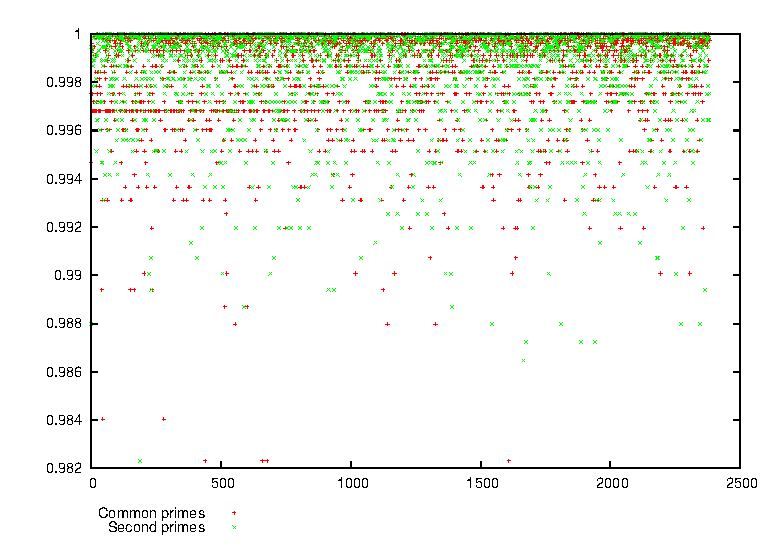
\includegraphics[width=16cm]{images/entropyprimes.eps}
\caption[Entropie moyenne]{Entropie moyenne des facteurs communs : 0.998518 - Entropie moyenne des seconds facteurs : 0.998551}
\label{entropiePrime}
\end{figure}


\subsection{Tailles des clefs}
Dans nos résultats, nous pouvons constater que seules deux tailles de clefs apparaissent : 512 et 1024 bits. Voici les chiffres :


\begin{table}[H]
\centering
\begin{tabular}{|r|c|c|}
\hline
\textbf{}&\textbf{512 bits}&\textbf{1024 bits}\\
\hline
\textbf{Total}&2 345&318 558\\
\hline
\textbf{Vulnérables}&6 (0,26\%)&2 376 (0,75\%)\\
\hline
\end{tabular}
\caption{Tailles de clefs obtenues}
\label{tailles}
\end{table}


Nous avions également d'autres tailles de clefs en entrée mais leur nombre devait être trop petit par rapport à l'espace des clefs de cette taille pour obtenir des facteurs communs.



\chapter{Analyse Statique : audit d'OpenSSL}

\section{But de cette partie}
Nous nous sommes concentrés sur les parties qui peuvent être critiques : 
\begin{description}
	\item [l'entropie :] un des problèmes les plus épineux lors de la génération de clef ;
	\item [la génération des clefs : ] c'est sur elles que reposent la sécurité d'un système cryptographique. Si leurs secrets venaient à être découverts, un utilisateur malveillant pourrait s'en servir pour déchiffrer facilement les massages d'un tiers (les fonctions de chiffrements étant en théorie publiques et éprouvés) ;
	\item [le chiffrement et les protocoles :] des failles sont trouvées régulièrement dans certains protocoles, et les avancées technologiques tendent aussi à rendre les algorithmes obsolètes (augmentation de la puissance de calcul des machines) ;
	\item [les signatures et les authentifications : ] les certificats et les signatures électroniques ont une importance particulière dans la sécurité protocolaire, et le mécanisme est souvent transparent à l'utilisateur ;
	\item [les protocoles SSL et TLS : ] OpenSSL est basé directement sur le protocole SSL puis ensuite sur celui de TLS (successeur de SSL).\\
\end{description}
Cette deuxième partie est un très court résumé du rapport d'audit réalisé pendant le projet. Pour de plus amples informations, nous vous conseillons de le consulter. Il est accessible sur le site web, onglet "Audit d'OpenSSL", et sur le git \cite{notregit}.

\subsection{Entropie}

L'entropie est la base pour générer des nombres pseudo-aléatoires. Elle joue donc un rôle prépondérant dans la sécurité de la cryptographie qui sera mise en place. Son générateur est composé de trois principaux éléments : 
\begin{description}
	\item [le bruit source : ] il doit être non déterministe, et renvoie de façon aléatoire des bits grâce à des processus non déterministes;
	\item [le composant de conditionnement : ] il permet d’augmenter ou de diminuer le taux d’entropie reçu;
	\item [une batterie de tests : ] elle fait également partie intégrante du système. Des tests sont réalisés pour déterminer l’état de santé du générateur aléatoire, permettant de s’assurer que la source d’entropie fonctionne comme attendu.\\
\end{description}

Plusieurs standards parlent de l'entropie, dont principalement la RFC 4086 \cite{rfc4086} et le FIPS 140 \cite{fips140-1} \cite{fips140-2}. Mais malgré les recommandations, quelques failles ont étés trouvées.\\

\textit{Nous vous invitons à vous référer au rapport d'audit, chapitre 2, pour de plus amples informations} 

\subsection{Génération des clefs}

Les clefs cryptographiques ont un rôle fondamental en cryptographie. En effet, elles sont censées être le seul secret à garder précieusement par leur possesseurs : il est conseillé que les algorithmes et tous les outils ne soient pas secret afin d'être certain de ne pas insérer de faille. Les algorithmes reconnus et éprouvés \textbf{exigent} la fiabilité contrairement aux algorithmes secrets et personnels.\\

Par conséquent les clefs se doivent d'être les plus solides possible. Mais malgré le soin qu'on peut y apporter, et les différentes recommandations qui sont faites par les normes, le risque zéro n'existe pas.\\

\textit{Nous vous invitons à vous référer au rapport d'audit, chapitre 2, pour de plus amples informations} 

\subsection{Chiffrement et protocoles}
De nombreux protocoles de chiffrement existent : 
\begin{itemize}
	\item symétrique :
	\begin {itemize}
		\item AES ;
		\item Blowfish ;
		\item DES ;
		\item 3-DES ;
		\item etc.\\
	\end{itemize}
	\item asymétrique : 
	\begin {itemize}
		\item DSA ;
		\item El Gamal ;
		\item RSA ;
		\item etc.\\
	\end{itemize}
\end{itemize}

RSA étant l'un des algorithmes les plus utilisés en cryptographie asymétrique, et étant limité dans le temps, nous nous sommes concentrés sur celui-ci.\\
Cependant, RSA seul n'est plus d'une sécurité absolue. Il peut-être est combiné par exemple à OAEP (RSA-OAEP). Un bourrage (\textit{padding}) est alors rajouté avant l'application de RSA. La norme principale qui se charge des recommandations sur RSA est la PKCS\#1, qui a aussi le nom de RFC 3447 \cite{3447} \cite{rfc3447_trad}.\\

\textit{Pour plus d'informations, nous vous invitons à aller consulter le rapport d'audit, chapitre 3} 

\subsection{Signature et authentification}
La signature électronique est de plus en plus utilisée, de façon plus ou moins transparente. Un mécanisme complexe est mis en place derrière, avec toute une chaîne d'autorités de certification et de révocation des certificats, ce qui permet de définir le niveau de fiabilité du certificat. \\
Processus de signature : 
\begin{figure}[H]
\begin{center}
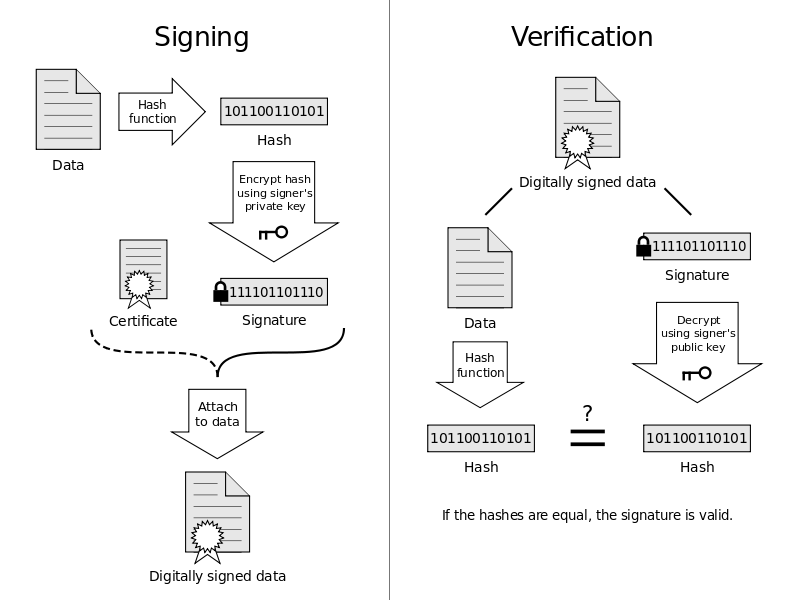
\includegraphics[width=10cm]{images/sig_dig.png}
\end{center}
\caption{Signature électronique}
\label{digital sig}
\end{figure}

La RFC 3447 \cite{rfc3447} \cite{rfc3447_trad} apporte aussi des recommandations à ce propos, ainsi que la RFC 979 \cite{rfc979}.\\

\textit{Pour consulter les principales failles que nous avons trouvées à ce sujet, nous vous invitons à aller consulter le rapport d'audit, chapitre 4} 

\subsection{Protocole SSL/TLS}
SSL et TLS (successeur de SSL) sont des protocoles de sécurisation des échanges sur internet. Les versions 2 et 3 de SSL ont été développées par Netscape puis le brevet a été racheté par l’IETF en 2001, qui a ensuite publié une évolution de ce protocole : TLS. Ce protocole fonctionne selon un mode client-serveur et fournit les objectifs de sécurité suivants :
\begin{itemize}
	\item authentification serveur/client;
	\item confidentialité des données échangées;
	\item intégrité des données échangées.\\
\end{itemize}
Du point de vue réseau, ce protocole se situe dans la couche session du modèle OSI et entre transport et application dans le modèle TCP.\\

\textit{Pour de plus amples informations, nous vous invitons à aller consulter le rapport d'audit, chapitre 5.}




















\chapter{Analyse dynamique}

\section{Objectifs}
L'objectif de ce projet consiste à étudier le comportement d'une machine cliente lorsqu'elle se connecte en SSL/TLS sur un serveur. Bien qu'à la base considéré comme optionnel, nous avons décidé de développer ce projet car nous avions de l'avance sur les parties précédentes. \\

Nous avons codé un serveur permettant d'analyser les différentes \textit{ciphersuite} utilisées à l'établissement de connexion d'un client à un serveur, et d'établir un diagnostique sur la qualité des suites utilisées par le client. Pour rappel, une \textit{ciphersuite} est une combinaison de noms pour l'authentification, le chiffrement, et les algorithmes MAC utilisés pour négocier les paramètres de sécurité pour une connexion réseau par TLS (\textit{Transport Layer Security})/ SSL (\textit{Secure Sockets Layer}). La structure de ces suites est définie dans la RFC 5246 \cite{rfc5246} et fut également décrite dans le rapport d'audit d'OpenSSL (Chapitre 5, Protocoles SSL/TLS).\\



La figure \ref{systServer} illustre le système à mettre en place.
\begin{figure}[H]
	\begin{center}
	
\includegraphics[scale=0.2]{images/logo_univ.png}
	\end{center}
\caption{Système Client/Serveur d'analyse SSL/TLS}
\label{systServer}
\end{figure}



\section{Mise en place du serveur}
\subsection{Exigences}
Il convient de pouvoir identifier les caractéristiques de la connexion entre le client et le serveur à savoir :
\begin{itemize}
\item la version du protocole mise en œuvre ;
\item les \textit{ciphersuites} proposées par le client ;
\item les courbes elliptiques supportées ;
\item les algorithmes de signature ;
\item la compression TLS, qui permet de compresser les données chiffrées afin d'accélérer le transfert de celles-ci ;
\item l'activation ou non du ticket de session.\\
\end{itemize}

Suivant ces caractéristiques, nous pouvons émettre un jugement sur la qualité du client SSL/TLS utilisé. Si un client possède des attributs étant considérés comme vulnérables, alors il faut pouvoir les identifier rapidement sur le site, et expliciter les raisons de l'affaiblissement du système.  


\subsection{Faiblesses à identifier}
\subsubsection{Version du protocole}
Si le client utilise une version \texttt{TLS 1.0} ou \texttt{SSLv3}, alors celui-ci sera considéré comme non sécurisé.\\

\begin{enumerate}
\item La version \texttt{SSLv3} précède la version \texttt{TLS 1.0} ; elle est considérée comme non sûre de nos jours. 

 
\item La version \texttt{TLS 1.0} est la toute première version de TLS, et demande une pré-configuration client et serveur importante pour être utilisé de façon sécurisée. De plus, cette version ne permet pas d'utiliser les dernières \textit{ciphersuites} récentes offrant une meilleure sécurité. De plus, cette version est vulnérable à l'attaque BEAST	(\textit{Browser Exploit Against SSL/TLS}).

\item Enfin, la version \texttt{TLS 1.1}  n'étant pas la dernière version TLS, nous considérons qu'elle est moyennement sûre.\\
\end{enumerate}



\subsubsection{Ciphersuites}
Nous avons pu identifier toutes les \textit{ciphersuites} étant considérées comme peu sûres, à savoir :
\begin{itemize}
\item les \textit{ciphersuites} utilisant des clés de taille inférieure à 128 bits pour le chiffrement ;
\item les \textit{ciphersuites} ne spécifiant aucun chiffrement pour la connexion ; 
\item les \textit{ciphersuites} sans authentification serveur, rendant l'attaque d'homme par le milieu possible ;
\item autres \textit{ciphersuites} étant supposées arrêtées après SSL 3.0, ou dont les caractéristiques de sûreté ne sont pas connues.
\end{itemize}


\subsubsection{Courbes elliptiques}
La RFC 5430 \ref{rfc5430} décrit deux niveaux de sécurité pour les courbes elliptiques, les clés de 128 bits et le cles de 192 bits, référencés sur le tableau \ref{ciphsuiteSec}. 

\begin{table}[H]
\centering

\begin{tabularx}{13cm}{|l|X|}
\hline
\textbf{\textit{Ciphersuite}} & \textbf{Niveau de sécurité} \\
\hline
\verb+TLS_ECDHE_ECDSA_WITH_AES_128_GCM_SHA256+ & 128\\
\verb+TLS_ECDHE_ECDSA_WITH_AES_128_CBC_SHA256+ & 128\\            
\verb+TLS_ECDHE_ECDSA_WITH_AES_128_CBC_SHA+    & 128\\            
\verb+TLS_ECDHE_ECDSA_WITH_AES_256_GCM_SHA384+ & 192\\            
\verb+TLS_ECDHE_ECDSA_WITH_AES_256_CBC_SHA384+ & 192\\            
\verb+TLS_ECDHE_ECDSA_WITH_AES_256_CBC_SHA+    & 192\\
\hline
\end{tabularx}

\caption{Niveaux de sécurité pour les \textit{ciphersuites}}
\label{ciphsuiteSec}
\end{table}


La RFC recommande l'utilisation de deux courbes :
\begin{itemize}
\item pour un niveau de sécurité à 128 bits, la courbe \texttt{secp256r1};
\item pour un niveau de sécurité à 192 bits, la courbe \texttt{secp384r1}.
\end{itemize}



\subsubsection{Compression des données chiffrées}
La compression des données chiffrées permet d'accélérer le transfert des données. Toutefois, cette technique permet à un attaquant d'effectuer une attaque de type CRIME (\textit{Compression Ratio Info-leak Made Easy}), qui permet de récupérer des données de session. %


\subsubsection{Ticket de session}
Les tickets de session permettent d'accélérer la reprise de communication chiffrée avec le serveur. Le temps de la poignée de main peut prendre du temps et ce ticket permet d'établir une session entre le client et le serveur. Lorsqu'un client se déconnecte puis se reconnecte avec un ticket de session, les échanges du \textit{handshake} sont passés, gagnant un temps considérable. 



\section{Implémentation}
Le serveur fut développé en C et il implémente les méthodes suivantes :
\begin{itemize}
\item \verb+sigaction+
\item \verb+get_version (SSL *ssl)+, qui retourne la version de connexion utilisée ; 
\item \verb+get_ecc_list (SSL *ssl)+, qui retourne la liste des courbes elliptiques ; 
\item \verb+get_cipher_suite_string(SSL_CIPHER *c)+, qui retourne un \textit{ciphersuite} à un état donné ; 
\item \verb+get_cipher_suite_list(SSL *ssl)+, qui permet l'affichage de tous les \textit{ciphersuites} ; 
\item \verb+get_sig_algs(SSL *ssl)+, qui renvoie les algorithmes de signature ; 
\item \verb+get_analyze_page(SSL *ssl)+ qui permet l'affichage global de la page ;
\item \verb+handle_connection(void * param)+  qui gère globalement la connexion entre le serveur et le client ;
\item \verb+new_thread(SocketTCP *socket)+ .
\end{itemize}





\begin{figure}[H]
\begin{center}

\includegraphics[scale=0.2]{images/logo_univ.png}
\end{center}
\caption[Exemple 1]{Exemple de figure avec titre raccourci}
\label{fig1}
\end{figure}


\begin{table}[H]
\centering
\begin{tabularx}{17cm}{|l|l|l|X|l|}
\hline
\textbf{Identifiant} & \textbf{KeyExch} & \textbf{Authn}& \textbf{Enc}& \textbf{MAC}\\
\hline
\verb+TLS_SRP_SHA_WITH_3DES_EDE_CBC_SHA+&SRP SHA1&SRP SHA1&3DES CBC&SHA1\\
\hline
\end{tabularx}
\caption{Exemple tableau}
\label{tableauEx}
\end{table}


\chapter{Vie de projet}
\section{Présentation de l'équipe}

Notre équipe est formée de cinq membres, tous étudiants à l'université de Rouen, dont un est également étudiant à l'INSA.
La définition des rôles s'est faite assez rapidement, nous souhaitions changer de rôle par rapport au projet de l'année dernière, afin de mieux explorer la gestion de projet.
Nous avons donc désigné Pascal Edouard comme chef de projet, Julien Legras comme Responsable technique, Claire Smets comme responsable client, et deux testeurs William Boisseleau et Mathieu Latimier.
Le choix des deux testeurs vient  du grand nombre de tests sur notre projet. Les résultats devant être sans faille.

Bien que chacun ait un rôle attitré, tous contribuent à différentes tâches du projet (tâches de développement, d'études, de tests, d'interfaces, etc...).

\section{Le client}

M. Otmani est notre client pour ce projet. Le cahier des charges se divise en trois grandes parties, pour la première, le client attend de nous un audit de clefs cryptographiques solide, présentable, et intuitif. Pour cela, il nous a conseillé d'étudier un article publié par des universitaires de Californie et du Michigan, ainsi que le site factorable.net.
Pour la seconde partie, nous devions faire un audit du code source d'OpenSSL par rapport aux normes prescrites (ex: RFC, PKCS, NIST, ...)
Le client souhaite notamment que l'on étudie la génération d'aléa, la génération des clefs, et le chiffrement.
Enfin, dans la dernière partie, le client nous propose d'établir un diagnostic de connexion entre un client et un serveur sur plusieurs critères comme la génération des nonces, la génération de la clef primaire, le contrôle des certificats, le respect du protocole, le choix de l'algorithme etc.

Cette dernière partie est optionnelle, elle sera effectuée si le temps nous le permet.

Le projet se déroule sur six semaines, le temps de travail est de 8h/jour (pour pouvoir palier le temps perdu par chacun pour la recherche de stage, les charges administratives, etc...)

\section{Méthode agile : SCRUM}

Nous avons choisi d'utiliser la méthode de développement agile SCRUM (comme indiqué dans le Plan de Développement) afin d’apporter une discipline de développement et de délivrer les résultats dans les meilleures conditions.\\
Dans ses sous-parties nous allons revenir sur le choix de la méthode, puis nous allons détailler son application tout au long du projet.

\subsection{Pourquoi Scrum ?}

Les méthodes agiles ont fait leur preuve dans leur efficacité et leur qualité de développement. De plus, Scrum permet un suivi et une transparence totale avec le client. Le découpage en sprints est adapté à notre projet puisqu’il se déroule en différentes parties et sur une période relativement courte.

\subsection{Valeurs et principes}

\paragraph{Les individus et leurs interactions plus que les processus et les outils} : la méthodologie Scrum correspond à la communication entre les collaborateurs à tous les niveaux (client/fournisseurs, testeurs/programmeurs, ...) afin de ne pas perdre de temps ni d’énergie avec des malentendus ou de l’incompréhension.\\

Cette valeur a été primordiale pour nous, la force de notre projet réside dans cette bonne communication entre chacun des membres.
Nous avons ainsi pu :
\begin{itemize}
\item détecter rapidement les problèmes avec de bonnes phases de tests, des réunions techniques en cas de doute, ...;
\item rentrer efficacement dans les sujets les plus importants du projet, surtout pour la partie de l'audit de code OpenSSL;
\item exposer efficacement nos travaux au client, les possibilités qui s'offrent à nous pour mieux satisfaire ses besoins;
\item nous mettre tous à niveau sur chaque partie en résumant le travail de chacun lors de chaque réunion.\\
\end{itemize}


\paragraph{La collaboration avec les clients plus que la négociation contractuelle} : une approche directe avec le client qui se sent beaucoup plus impliqué dans le projet afin qu’il puisse apporter ses avis et remarques.\\

Nous sommes partis du principe que le client faisait partie intégrante de l'équipe. Son avis nous intéressant, nous lui avons montré lors de toutes nos réunions nos travaux afin qu'il puisse s'assurer du bon avancement du projet et qu'il puisse nous aiguiller pour la suite.\\
De plus, nous évitions au maximum de faire des livraisons ou des demandes au client par messagerie électronique, préférant des rencontres interpersonnelles.


\paragraph{L’adaptation au changement plus que le suivi d’un plan} : être capable de s’adapter lorsqu’une modification importante est nécessaire.\\

Nous sommes partis d'un but général fixé sans détailler les étapes de chaque tâche afin de laisser libre cours au changement de contexte, aux risques pouvants être rencontrés, aux sujets que le client souhaitait plus appronfondir, etc...\\
Les livraisons correspondent donc aux besoins du client, et sont modulables afin d'appronfondir l'étude.

\subsection{Réunions}

\subsubsection{Brainstorming et Stand-Up Meeting}

Chaque matin tout le monde se réunit autour d'un café, et partage son ressenti sur le projet, et sur les tâches à venir. Ici, rien de technique, nous contrôlons juste la bonne avancée de chacun, et la compréhension générale du projet. \\
C'est également le bon moment pour définir les dates des prochaines réunions techniques.\\
Ces réunions s'apparentent aux "Mélées Quotidiennes" du SCRUM.

\subsubsection{Réunions hebdomadaires}

Nous nous réunissons deux fois par semaine, le jeudi.
En début d'après-midi, ou en fin de matinée, nous passons dans une salle au calme, pour parler des difficultés techniques rencontrées, des axes d'améliorations, de la réorganisation ou du découpage des tâches si besoin.\\
Nous évoquons également les points importants à apporter au client pour la réunion qui suit.\\
Ces réunions s'apparentent aux "Planifications du Sprint" et à la "Rétrospective de Sprint" du SCRUM.

L'après-midi, selon la disponibilité du client, nous nous réunissons pour parler de notre avancée, relever les remarques et les envies du client, présenter nos résultats ou livrer une partie de projet finie.\\
Ces réunions s'apparentent aux "Revue de Sprint" du SCRUM.

\subsubsection{Réunions d'urgences}

Plus rarement, il a pu nous arriver d'avoir des réunions d'urgence. Nous nous sommes ainsi réunis avec le client lorsque nous étions bloqués sur la récupération des certificats SSH, ou lorsque l'on s'est aperçus qu'une amélioration majeure était possible.

\subsubsection{Audit}

Les audits avec M. Abdellah Godard, nous ont permis d'avoir des remarques pertinentes sur nos documents livrables, et de progresser dans notre méthodologie de gestion de projet. Nous avons ainsi amélioré nos outils de gestion de projet, par exemple en passant notre planning sur le GantterProject afin de mieux visualiser les tenants et les aboutissants d'une tâche, et perfectionner nos documents livrables notamment au niveau de la traçabilité.

\section{Outils pour la gestion de projet}

Durant ces six semaines de travail, nous avons eu l'occasion de tester plusieurs logiciels outils pour notre projet.

\subsection{Git}

Git est un logiciel libre de gestion de versions décentralisé, créé par Linus Torvalds en 2005, accessible sur les systèmes Linux et Windows.\\
Un logiciel de gestion de versions est un logiciel qui permet de stocker un ensemble de fichiers en conservant la chronologie de toutes les modifications qui ont été effectuées dessus. Il permet notamment de retrouver les différentes versions d’un lot de fichiers connexes.\\
Lorsqu'un membre a terminé sa tâche, il ajoute les fichiers modifiés sur la branche concerné, en placant un commentaire pour expliquer les modifications apportées.\\
Il est ensuite plus simple de voir les différences entre chaque version, et de retrouver une ancienne version si besoin.\\

\subsection{Redbooth}

Redbooth (anciennement Teambox) est un outil de gestion de projet en ligne pour des équipes de quelques membres. Il nous permet de suivre l'évolution des tâches : en cours de réalisation et celles à venir. Ces tâches peuvent être de différentes sortes :
\begin{itemize}
\item tâches du projet;
\item tâches de gestion de projet (outils, documents livrables);
\item tâches pour la gestion des réunions (comptes-rendus, livraisons, signatures, ...);
\item autres tâches (ex : recherche d'informations sur le choix des langages de développements, état de l'art, analyse de documents spécifiques).\\
\end{itemize}

\subsection{Google drive}

Google Drive est un service clourd proposé par google en 2012 pour le stockage et le partage de fichier.\\
C'est une bonne alternative au Git, qui nous permettait de partager des ressources sous toutes formes (articles, logiciels, scripts), et nos résultats en vrac afin de pouvoir les tester sur nos machines (listes d'adresses IP, certificats, fichiers d'insertion en base de données, etc.)\\
Une fois les fichiers validés ils pouvaient être déplacés vers le Git si l'on pensait qu'ils avaient une importance pour le projet final.\\
Il nous permettait également de synchroniser nos résultats notamment lors de notre état de l'art pour la partie 2 du projet.

\subsection{Google Hangouts}

Hangouts est une plate-forme de messagerie instantanée qui nous permettait de partager nos ressentis, d'indiquer notre progression sur une tâche aux autres, proposer de l'aide si besoin.\\
Ce service est très utile car il nous permettait également de rester sur la même plate-forme que le Drive et nos mails, ce qui était un gain de temps non négligeable.

\subsection{GanttProject et GantterProject}

Gantter est une application outil pour le management de projet basé sur le web (que l'on peut d'ailleurs consulter sur le GoogleDrive)
Nous avons tout d'abord réalisé notre diagramme de Gantt avec GanttProject, mais il s'avérait qu'il fallait calculer les informations demandées par l'auditeur (qui jouait le rôle du client).\\
Parmis les informations non-visibles sur un diagramme réalisé avec GanttProject que l'on trouve sur un GantterProject nous avons :
\begin{itemize}
\item
\end{itemize}

De plus, le diagramme du GantterProject est plus esthétique que notre précédent diagramme, ce qui nous permettait de retrouver plus facilement nos informations.

\subsection{LaTeX et BibTeX}

Latex est un langage de structuration de document créé en 1983 par Leslie Lamport. Il utilise des macro-commandes qui seront interprétés par un processeur de texte TeX.\\
Bibtex est un logiciel de gestion de références bibliographiques qui nous a servi à gérer et traiter notre base bibliographique à travers nos documents Latex.\\

Nous avons choisi de réaliser l'ensemble de nos documents (comptes-rendus, rapports, livrables) sous LaTeX pour qu'ils soient homogènes (nous partions sur la même base), réutilisables et modulables (découpage sous forme de briques).

Les éditeurs/compilateurs de LaTeX sont nombreux, nous avons opté pour deux d'entres eux : Gummi et TexMaker.

\section{Tests}

Pour nos tests nous avons eu besoin de quelques outils que nous détaillons ci-dessous.

\subsection{Ressources de Tests}
\subsubsection{Netkit}

Netkit est un environnement permettant de configurer et de tester un réseau virtuel rapidement et sans grandes ressources.\\
Lors des procédures de tests de la première partie, nous voulions générer un petit réseau comportant toutes les configurations possibles rencontrables lors du scan, de la récupération de certificats et de la post-récupération (extraction de données, gestion des doublons, liens symboliques, etc...).\\
Nous avons donc décidé de réaliser ce petit réseau à l'aide de l'outil Netkit.

\subsubsection{Pencil}

Pencil est un logiciel de création de maquettes typographiques libre et gratuit développé par Evolution Solutions.
Nous nous sommes servis de ce logiciel afin de réaliser les maquettes des pages web attendues pour chacune des trois parties.\\
Le rendu final n'est pas exactement celui des maquettes car nous avons également utilisé plusieurs frameworks pour améliorer la qualité graphique (i.e. HighCharts, BootStraps), mais le contenu et la disposition est sensiblement la même.
Ces tests nous ont permis de partir sur une base commune.

\subsection{Procédures de tests}

Pour la configuration du réseau minimaliste, possédant différentes configurations que nous pourrons rencontrer lors du scan, puis de la récupération du certificat, les différentes configurations sont les suivantes :
\begin{itemize}
\item une machine avec un certificat SSL présent et valide
\item une machine avec un certificat SSL présent et révoqué
\item une machine avec un certificat SSL modifié (donc incorrect)
\item une machine avec un certificat SSL présent et valide mais doublé
\item une machine avec un certificat SSL présent et valide, mais tournant sur un autre port que 443
\item une machine avec un certificat SSL présent et valide avec changement de configuration (tests sur la 1e machine - SSLCiphers, SSLProtocols, ...)
\end{itemize}

Pour créer un certificat d'autorité SSL :
\begin{itemize}
\item On génère un couple clé privée, clé publique RSA de 1024 bits\\
\begin{verbatim}
openssl genrsa 1024 > cert.key
\end{verbatim}
\item On créer un certificat auto-signé (peu nous importe la nature du certificat ici) - ce sera notre certificat racine\\
\begin{verbatim}
openssl req -new -x509 -days 365 -key cert.key > cert.crt
\end{verbatim}
\item Ensuite, on fait une demande de certificat auprès du certificat autorité\\
\begin{verbatim}
openssl req -new -key test.key > test.csr
\end{verbatim}
\item Enfin, on peut signer ce dernier avec notre certificat racine\\
\begin{verbatim}
openssl x509 -req -in test.csr -out test.crt -CA cert.crt -CAkey cert.key -CAcreateserial -CAserial cert.srl
\end{verbatim}
\end{itemize}

Pour révoquer un certificat :
\begin{itemize}
\item 
\begin{verbatim}
openssl ca -revoke test.crt -cert test.crt -keyfile test.key -config openssl.cnf
\end{verbatim}
\item 
\begin{verbatim}
openssl ca -gencrl -config openssl.cnf -crldays 7 -out listcrl.crl
\end{verbatim}
\end{itemize}

Il ne faut pas oublier de concaténer les certificats, il sera nécessaire dans la configuration de notre serveur web :
\begin{itemize}
\item 
\begin{verbatim}
cat test.crt cert.crt > concatcert.crt
\end{verbatim}
\end{itemize}

Pour ce qui est de la preuve de F, nous avons un jeu de tests avec des arbres comportant un nombre de nœuds impairs ou pairs, et comportant des nombres premiers communs ou non.

\section{Ressources techniques}

Pour ce qui est du développement de scripts, de la gestion du site web avec base de données et de la mise en place du navigateur sécurisé de la troisième partie nous avons utilisé les machines de l'université et nos ordinateurs portables. Mais pour les parties plus délicates comme le scan de ports Internet, la récupération de certificats ou la factorisation des moduli pour la première partie nous avions des ressources techniques plus importantes.

\paragraph{Connexion internet : } pour la première partie, nous avions besoin d'une bonne connexion internet pour le scan, ainsi que pour la récupération des certificats. Il fallait prendre certaines précautions afin de ne pas congestionner le réseau, et éviter également que le proxy ne dérange le déroulement des scripts. Ainsi nous avons lancé les scans importants les vendredi soirs, en utilisant la prise ethernet extérieur.

\paragraph{Serveur de calcul de l'Université :} ce serveur nous a permis de factoriser les moduli lors du deuxième scan (plus conséquent - environ 500 000 certificats), et de gagner du temps sur l'avancement de notre projet.

\section{Choix des langages de développement}

\subsection{Langage C et librairie GnuMP}

Nous avons décidé avant de débuter le projet de faire une étude en benchmark-test \cite{chooseprogram2013} \cite{marceau2009program} \cite{udemypng} (test de performance CPU, RAM, taille de code), sans oublier deux principes fondamentaux qui sont la gestion des grands entiers et les préférences de chacun (degré de compétence, aisance).\\
Les codes sont basés sur l'utilisation combinée de structures et d'algorithmes complexes (sur arbres, ensembles, anneaux, etc...).\\

Plusieurs langages ont étés testés parmis lesquelles :
\begin{itemize}
\item C;
\item C++;
\item Java;
\item Perl;
\item Python;
\item Ruby.\\
\end{itemize}

Nous avons au final décidé d'utiliser le langage C avec la librairie GnuMP \cite{gmplib} pour la gestion des grands entiers, et le compilateur CMAKE.
Le langage C est l'un des plus rapides en temps d'exécution, il est également l'un de ceux qui consomment le moins de mémoire. Il est également très performant sur la gestion des grands entiers.\\
Le python et le C++ étaient également de très bons choix, mais les développeurs ont une meilleure maîtrise du C.

\subsection{Langages de scripts : Bash et Perl}

\subsection{IDE : Eclipse}

\section{IHM}

\subsection{Langage Web : HTML5, CSS, PHP, Javascript, AjaX, JQuery}

\subsection{Design avec BootStrap}

\subsection{Doxygen}

\subsection{Base de donnée : MySQL}

\section{Gestion des risques}

\addcontentsline{toc}{section}{Conclusion}
\section*{Conclusion}

Conclusion rapport final 




{\small
\bibliographystyle{acm}
\bibliography{references}
}

\end{document}